\exercise{6\textbar 1}{Gleichgewicht am Markt für Speiseeis}

\textbf{Aufgabe:}  
Stellen Sie sich vor, dass in einer kleinen deutschen Stadt ein harter Konkurrenzkampf auf dem Markt für italienisches Speiseeis tobt.  

\begin{enumerate}[label=\alph*)]
    \item Das Angebot der zahlreichen Eisdielen ist beschrieben durch folgende Funktion: $p^a(x) = 2 + 0,1x$.
    \item Die Nachfrage, die vor allem durch die Studierenden der Stadt entfaltet wird, ist gegeben durch: $p^n(x) = 12 - 0,1x$.
\end{enumerate}

Da Sie selbst häufig Eisdielen besuchen, haben Sie sich vorgenommen, diesen Markt einmal etwas genauer unter die Lupe zu nehmen:

\begin{enumerate}[label=\alph*)]
    \item Berechnen Sie nun zunächst den markträumenden Preis sowie die gleichgewichtige Menge für italienisches Speiseeis.
    \item Wie hoch sind die Produzentenrente und die Konsumentenrente? Skizzieren Sie die Lösung!
\end{enumerate}

\solution{

\begin{enumerate}[label=\alph*)]
    \item \textbf{Markträumender Preis und gleichgewichtige Menge:}
    \begin{itemize}
        \item Im Marktgleichgewicht muss gelten, dass das aggregierte Angebot der aggregierten Nachfrage entspricht:
        \[
        p^a(x) = p^n(x)
        \]
        \item Setzen der Funktionen:
        \[
        2 + 0,1x = 12 - 0,1x
        \]
        \item Auflösen nach $x$:
        \[
        0,2x = 10 \implies x = 50
        \]
        (Das ist die \textbf{gleichgewichtige Menge}!)
        \item Der \textbf{markträumende Preis} kann auf zwei Arten berechnet werden:
        \[
        p^a(50) = 2 + 0,1 \cdot 50 = 7
        \]
        oder
        \[
        p^n(50) = 12 - 0,1 \cdot 50 = 7
        \]
    \end{itemize}
    \item \textbf{Konsumentenrente und Produzentenrente:}
    \begin{itemize}
        \item Konsumentenrente:
        \[
        \text{Konsumentenrente} = (12 - 7) \cdot 50 \cdot 0,5 = 125 \, \text{€}
        \]
        \item Produzentenrente:
        \[
        \text{Produzentenrente} = (7 - 2) \cdot 50 \cdot 0,5 = 125 \, \text{€}
        \]
    \end{itemize}
\end{enumerate}

\begin{figure}[H]
    \centering
    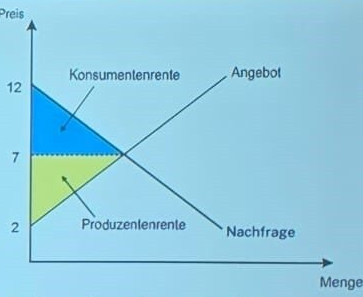
\includegraphics[width=0.5\textwidth]{figures/6_1.png}
    \caption{Marktgleichgewicht von Angebot und Nachfrage für Speiseeis}
    \label{fig:ice_market}
\end{figure}
}
\exercise{6\textbar 2}{Schocks am Markt für Speiseeis}

\textbf{Aufgabe:}  
In diesem Jahr haben zahlreiche Ereignisse Einfluss auf den Markt für italienisches Speiseeis genommen:

\begin{itemize}
    \item Eine neue Fachhochschule wird eröffnet.
    \item Der Preis für Langnese-Eis sinkt.
    \item Der Stundenlohn für Eisverkäufer steigt aufgrund gestiegener Krankenkassenbeiträge.
    \item Die Hygieneanforderungen werden verschärft.
    \item Die BAföG-Sätze werden gesenkt.
\end{itemize}

Skizzieren Sie jeweils die Effekte, die hiervon auf die Angebots- und Nachfragekurve ausgehen!

\solution{

Die Lösung visualisiert die Auswirkungen auf Angebots- und Nachfragekurven in den gegebenen Szenarien. Die entsprechenden Diagramme sind in Abbildung \ref{fig:ice_market_shocks} dargestellt.

\begin{figure}[H]
    \centering
    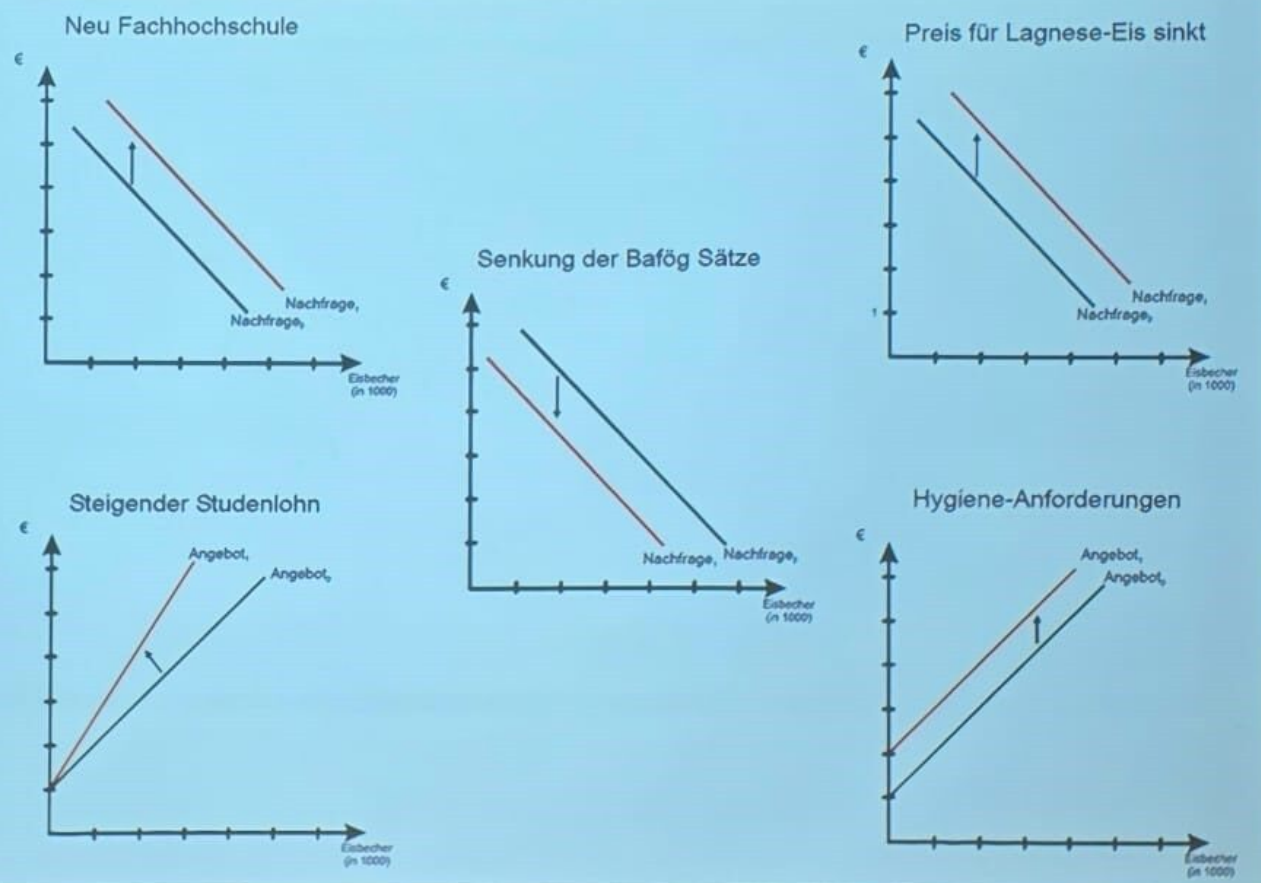
\includegraphics[width=0.8\textwidth]{figures/6_2.png}
    \caption{Einfluss verschiedener Schocks auf den Markt für Speiseeis}
    \label{fig:ice_market_shocks}
\end{figure}
}

